\def\year{2021}\relax
%File: formatting-instructions-latex-2021.tex
%release 2021.2
\documentclass[letterpaper]{article} % DO NOT CHANGE THIS
\usepackage{aaai21}  % DO NOT CHANGE THIS
\usepackage{times}  % DO NOT CHANGE THIS
\usepackage{helvet} % DO NOT CHANGE THIS
\usepackage{courier}  % DO NOT CHANGE THIS
\usepackage[hyphens]{url}  % DO NOT CHANGE THIS
\usepackage{graphicx} % DO NOT CHANGE THIS
\usepackage{amsmath}
\usepackage{amssymb}
\usepackage{gensymb}
\usepackage{hyperref}
\urlstyle{rm} % DO NOT CHANGE THIS
\def\UrlFont{\rm}  % DO NOT CHANGE THIS
\usepackage{natbib}  % DO NOT CHANGE THIS AND DO NOT ADD ANY OPTIONS TO IT
\usepackage{caption} % DO NOT CHANGE THIS AND DO NOT ADD ANY OPTIONS TO IT
\frenchspacing  % DO NOT CHANGE THIS
\setlength{\pdfpagewidth}{8.5in}  % DO NOT CHANGE THIS
\setlength{\pdfpageheight}{11in}  % DO NOT CHANGE THIS
%\nocopyright
%PDF Info Is REQUIRED.
% For /Author, add all authors within the parentheses, separated by commas. No accents or commands.
% For /Title, add Title in Mixed Case. No accents or commands. Retain the parentheses.
% /Title ()
% Put your actual complete title (no codes, scripts, shortcuts, or LaTeX commands) within the parentheses in mixed case
% Leave the space between \Title and the beginning parenthesis alone
% /Author ()
% Put your actual complete list of authors (no codes, scripts, shortcuts, or LaTeX commands) within the parentheses in mixed case.
% Each author should be only by a comma. If the name contains accents, remove them. If there are any LaTeX commands,
% remove them.

% DISALLOWED PACKAGES
% \usepackage{authblk} -- This package is specifically forbidden
% \usepackage{balance} -- This package is specifically forbidden
% \usepackage{color (if used in text)
% \usepackage{CJK} -- This package is specifically forbidden
% \usepackage{float} -- This package is specifically forbidden
% \usepackage{flushend} -- This package is specifically forbidden
% \usepackage{fontenc} -- This package is specifically forbidden
% \usepackage{fullpage} -- This package is specifically forbidden
% \usepackage{geometry} -- This package is specifically forbidden
% \usepackage{grffile} -- This package is specifically forbidden
% \usepackage{hyperref} -- This package is specifically forbidden
% \usepackage{navigator} -- This package is specifically forbidden
% (or any other package that embeds links such as navigator or hyperref)
% \indentfirst} -- This package is specifically forbidden
% \layout} -- This package is specifically forbidden
% \multicol} -- This package is specifically forbidden
% \nameref} -- This package is specifically forbidden
% \usepackage{savetrees} -- This package is specifically forbidden
% \usepackage{setspace} -- This package is specifically forbidden
% \usepackage{stfloats} -- This package is specifically forbidden
% \usepackage{tabu} -- This package is specifically forbidden
% \usepackage{titlesec} -- This package is specifically forbidden
% \usepackage{tocbibind} -- This package is specifically forbidden
% \usepackage{ulem} -- This package is specifically forbidden
% \usepackage{wrapfig} -- This package is specifically forbidden
% DISALLOWED COMMANDS
% \nocopyright -- Your paper will not be published if you use this command
% \addtolength -- This command may not be used
% \balance -- This command may not be used
% \baselinestretch -- Your paper will not be published if you use this command
% \clearpage -- No page breaks of any kind may be used for the final version of your paper
% \columnsep -- This command may not be used
% \newpage -- No page breaks of any kind may be used for the final version of your paper
% \pagebreak -- No page breaks of any kind may be used for the final version of your paperr
% \pagestyle -- This command may not be used
% \tiny -- This is not an acceptable font size.
% \vspace{- -- No negative value may be used in proximity of a caption, figure, table, section, subsection, subsubsection, or reference
% \vskip{- -- No negative value may be used to alter spacing above or below a caption, figure, table, section, subsection, subsubsection, or reference

\setcounter{secnumdepth}{0} %May be changed to 1 or 2 if section numbers are desired.

% The file aaai21.sty is the style file for AAAI Press
% proceedings, working notes, and technical reports.
%

% Title

% Your title must be in mixed case, not sentence case.
% That means all verbs (including short verbs like be, is, using,and go),
% nouns, adverbs, adjectives should be capitalized, including both words in hyphenated terms, while
% articles, conjunctions, and prepositions are lower case unless they
% directly follow a colon or long dash

% INSTRACTIONS FOR THE DEMO TRACK:
% An extended abstract of no more than 2 pages (including references) using the latest AAAI template. This should include the title of the proposed demonstration, the list of authors and their affiliations, and an abstract of up to 250 words. It should describe the technical content of the demonstration, with the appropriate credits and references. The abstract must include a link to a video file no more than 10 minutes long, hosted on a public service that allows streaming or downloading. The video of the demonstration is as important as the extended abstract for evaluating the suitability and merit of the proposed demonstration.

% A description of any non-standard hardware or software requirements or other requested logistical arrangements (within the confines of a virtual conference).

% The extended abstracts for accepted demonstrations will be available to conference participants and will be archived on the conference website.


% \title{Modeling Angry Birds in PDDL+}
\title{Playing Angry Birds with a Domain-Independent PDDL+ Planner}
% \author{Submission \#335}
\author{
    %Authors
    % All authors must be in the same font size and format.
    Wiktor Piotrowski,\textsuperscript{\rm 1}
    Roni Stern,\textsuperscript{\rm 1,2}
    Matthew Klenk,\textsuperscript{\rm 1}
    Alexandre Perez,\textsuperscript{\rm 1}
    Shiwali Mohan,\textsuperscript{\rm 1}
    Johan de Kleer,\textsuperscript{\rm 1}
    Jacob Le\textsuperscript{\rm 1}
    \\
}
\affiliations{
    %Afiliations
    \textsuperscript{\rm 1} Palo Alto Research Center, CA, USA\\
    \textsuperscript{\rm 2} Ben-Gurion University of the Negev, Beer-Sheva, Israel\\
    e-mail: \{wiktorpi,rstern,aperez,smohan,dekleer,jale\}@parc.com;klenk.matt@gmail.com\\
}
\begin{document}

\maketitle

\begin{abstract}
This demo paper presents the first system for playing  the popular Angry Birds game using a domain-independent planner.
Our system models Angry Birds levels using PDDL+, a planning language for mixed discrete/continuous domains. It uses a domain-independent PDDL+ planner to generate plans and executes them.
In this demo paper, we present the system's PDDL+ model for this domain, identify key design decisions that reduce the problem complexity, and compare the performance of our system to model-specific methods for this domain. The results show that our system's performance is on par with other domain-specific systems for Angry Birds, suggesting the applicability of domain-independent planning to this benchmark AI challenge.
A video explaining and demonstrating the behavior of our system is available at \texttt{https://bit.ly/35065UZ}.
\end{abstract}


% \section{Introduction}

%$Automated Planning in mixed discrete/continuous domains is an important hurdle to developing solutions for real world problems.

% What is Angry birds, why is it hard and "important"
\section{Background: Angry Birds}
Angry Birds is a wildly popular mobile game in which the objective is to destroy pigs by launching birds at them from a slingshot. The pigs may be protected by structures built from blocks of various types. Each level of the game has an allotted number of birds that can be used, and pigs that need to be killed in order to solve the level.
Players earn points by destroying pigs and blocks as well as for each unused bird after the level has been solved.
%Figures~\ref{fig:easy-level} and~\ref{fig:hard-level} illustrates two Angry Birds levels.
% Maybe say more here about the different levels and components
% \subsection{Viability as an AI Testbed}
This game is an interesting testbed for automated planning research since it
requires reasoning about sequential actions with complex dynamics~\cite{renz2019ai}.
% An intelligent agent playing Angry Birds needs to plan ahead and predict future states of the world, based on the agent's actions.
Unlike classical planning, the agent's actions often trigger a cascading chain of events causing drastic changes to the world.
The Angry Birds game is inherently a non-trivial hybrid system, exhibiting both discrete and continuous behavior, which includes non-linear dynamics.
Game levels often contain a large number of objects, which vary in their type and functionality.
%,and composite structures that includes different types of objects.
From a computational complexity perspective, different versions of the game have proven to be NP-Hard, PSPACE-complete, and EXPTIME-hard~\cite{stephenson2020computational},
% Why AI should not give up
% While the complexity of the full game can be at times overwhelming, Angry Birds provides a rich world for creating generalizable intelligent agents, and solving it would prove a significant milestone in Artificial Intelligence.
% All of the above points makes Angry Birds an important benchmark for the AI community and has driven researchers to create a clone of the game, called Science Birds\cite{renz2019ai}, for research purposes.
% Nevertheless, the reigning world champion is still a human.
% Our approach
Most existing AI agents for this game are based on encoding domain-specific strategies and selecting from them~\cite{borovicka2014datalab,wang2017description}.
We describe the first successful application of domain-independent planning to solve Angry Birds,
and demonstrate that its performance is on par with existing domain-specific approaches.


\section{Solving Angry Birds with a PDDL+ Planner}

% We modeled the problem using PDDL+ \cite{fox2006modelling}, which is a planning language that enables modeling problems exhibiting both discrete mode switches and continuous flows.


Our agent, called Hydra, models Angry Birds levels using PDDL+ \cite{fox2006modelling}. PDDL+ is a planning language that enables modeling problems exhibiting both discrete mode switches and continuous flows.
Hydra accepts an Angry Birds level from the Science Birds API~\cite{renz2019ai}, in the form of a list of labeled objects and their locations, and translates it to a PDDL+ problem.
Then, it solves this problem using  UPMurphi~\cite{della2009upmurphi}, a well-known domain-independent PDDL+ planner. %, which has that was used for problems in other domains~\cite{della2010pddl+}.

% Hydra works with the Science Birds API~\cite{renz2015aibirds}, which outputs a game level as a list of labeled objects and their locations.
% Hydra automatically translates this list into a PDDL+ problem. Then, it solves this problem using  UPMurphi~\cite{della2009upmurphi}, which is domain-independent PDDL+ planner that has been used for problems in other domains~\cite{della2010pddl}.



% \subsubsection{Modeling}
% that solves hybrid planning problems via a uniform discretization approach.
% , which encodes the relevant information about this level. To solve these PDDL+ problems, we used UPMurphi~\cite{della2009upmurphi}, which is domain-independent PDDL+ planner that solves hybrid planning problems via a uniform discretization approach.
% In order to use a domain-independent planning approach, it is necessary to select a modeling language.
% Most existing domain-independent planning languages, such a STRIPS \cite{fikes1971strips}, PDDL \cite{mcdermott1998pddl}, and PDDL2.1 \cite{fox2003pddl2}, lack features to capture Angry Birds.
% Most existing domain-independent planning languages lack features to capture Angry Birds. [no space :(]
% Therefore, we modeled the problem using PDDL+ \cite{fox2006modelling}, which is a planning language that is designed for mixed discrete/continuous domains. PDDL+ enables reasoning about ballistic flight of birds and the consequences of their collisions with objects.
% \subsubsection*{PDDL+}
%To date, the language with, arguably, the most set of features relevant to real-world problems is PDDL+~\cite{fox2006modelling}. It was designed specifically as a planning standard for modeling hybrid systems (switched dynamical systems) governed by a set of differential equations and discrete mode switches.
% Formally defined as a mapping of planning constructs to Hybrid Automata~\cite{henzinger2000theory},
% % Therefore,
% We modeled the problem using PDDL+ \cite{fox2006modelling}, which is a planning language that enables modeling problems exhibiting both discrete mode switches and continuous flows.
%PDDL+ supports continuous effects, timedPDDL+ builds on the expressiveness of its predecessors PDDL2.1 and PDDL2.2.
%, encapsulating the entire set of features from PDDL2.1 (including continuous effects)~\cite{} and supplements that with the inclusion of timed-initial literals (TILs) from PDDL2.2~\cite{}.  However, the biggest advancement over its predecessors is the inclusion of new constructs for defining exogenous activity in the domain.


% Recent works highlight how PDDL+ expressiveness teamed with clever system modeling can achieve high planning performance in a range of domains, including Urban Traffic Control~\cite{vallati-et-al:aaai-2016}, Chemical Batch Plant~\cite{della2010pddl+}, Minecraft~\cite{roberts2017automated}, and Atmospheric Re-entry~\cite{piotrowski2018heuristics}).
% The expressiveness of PDDL+ enables natural definitions of phenomena in Angry Birds.


% \noindent\textbf{Angry Birds Objects in PDDL+}
% Angry Birds is a difficult scenario to define as a planning domain. It contains a variety of distinct object types and complex interweaving dynamics\footnote{Our Angry Birds PDDL+ model relies on knowledge obtained from Angry Birds where possible. Beyond parameters we could reliably source, we approximate the behavior and parameters to the best of our knowledge via experiments and observations.}. However, PDDL+ facilitates the modeling of such constructs and their implementation.
The objects in our PDDL+ model of Angry Birds are separated into four types: \textit{birds, pigs, blocks, and platforms}.
Objects' properties such as locations, width, height, and velocities are modeled as functions. % in our model. % (AKA numeric fluents).
%, each one is a crucial component of the game and requires explicit representation. Note that
The slingshot, which is where the birds are launched from, is not modeled explicitly as an object in the domain. Instead, we assigned the slingshot's coordinates to every bird before it is launched.
Avoiding modeling unnecessary objects
simplifies planning. %the domain.
%helps in maintaining a light-weight domain definition. % \noindent\textbf{Birds} The only objects directly controlled by the player are the birds. Each bird object requires a set of numeric functions to accurately track their state, including XY coordinates, velocities, mass, bounce count (denoting the number of times the bird collided with any other object), and an ID number to keep the order in which the birds are launched. This set of functions is supplemented by a single predicate for each bird stating whether it has been released from the slingshot.
% \noindent\textbf{Pigs} %Pigs are simply targets in our PDDL+ model, they
% A pig is represented by its XY position, radius, and mass functions, as well as a single predicate stating whether it is alive. Pigs are mostly static entities in Angry Birds and their PDDL+ representation is a straightforward translation.
% \noindent\textbf{Blocks} The PDDL+ representation of blocks is very minimal. Each block is primarily defined by its basic characteristics, namely the XY coordinates, as well as the width and length values. Furthermore, blocks are also assigned values for mass, life-points, and stability (force needed to topple it), calculated based on the shape and size of the block, material (ice, wood, or stone), and what height it is positioned at (the taller a structure, the lower stability). Finally, each block is assigned a predicate dictating whether it is explosive to account for TNT crates. While there are different types of blocks in the Angry Birds game, we do not explicitly differentiate between them to keep the entire block ontology unified, and reduce unnecessary bloating of the domain.
% \noindent\textbf{Platforms} These Angry Birds elements are entirely static and indestructible, and modeled in PDDL+ via a pair of XY coordinates, supplemented by its width and height functions.
% \smallskip
% Finally, the model is supplemented by variables divided into two groups, global parameters and auxiliary operating parameters. The former includes important variables used globally in the system dynamics calculations, such as gravity, or launch angle and its rate of change. Auxiliary operating parameters are variables which play a supporting role such as denoting the currently active bird.
% The number of predicates and functions per object type in the domain is purposely limited in numbers to facilitate efficient planning and maintain readability. This design decision was motivated by mitigating a lower planning performance in Angry Birds levels which often contain a multitude of distinct objects. As described above, each object is defined in PDDL+ by a set of state variables. Densely populated levels can cause states to drastically increase in size (often containing hundreds of variables each), which, in turn, can lead to significant drop in planner performance.
% \noindent\textbf{Angry Birds Dynamics in PDDL+}
The PDDL+ domain of Angry Birds features a variety of dynamics which dictate the change and evolution of the system.
We modeled these dynamics through PDDL+ \emph{actions, events, and processes} constructs.
%Exogenous activities are expressed in PDDL+ as  \textit{discrete events} and \textit{continuous processes}.
PDDL+ events represent the system's mode switches which instantaneously change the dynamics of the modeled system, whereas PDDL+ processes represent processes that evolve the system over time, dictated by a set of ordinary differential equations.



% The PDDL+ domain of Angry Birds features a variety of dynamics which dictate the change and evolution of the system. This however, creates planning problems with vast search spaces and large branching factors, making them computationally difficult to solve. Thus, mitigating the issues of solvability and efficiency was at the forefront of the domain's development at each step of the process, and is evident in the resulting PDDL+ model's composition.

\noindent\textbf{Actions}
Angry Birds features two types of actions: (1) launching a bird from the slingshot at a chosen angle, and (2) activating a bird's special power (if available).
Currently, we only consider the basic behavior of birds without their special powers.
Launching of the bird consists of
choosing an angle, adjusting the launch velocity, and releasing the bird.
%This activity requires in-depth reasoning about the locations of the targeted structures, their strength and stability, and the force required to destroy or collapse them, in addition to the locations of pigs and other objects of interest (e.g. TNT crates).
%Encoding all of this information into actions would require complex constructs for each phase, and would result in concurrent and entangled behavior to account for both the angle and initial launch velocity.
%To mitigate the complexity of the launch action, we leverage the expressiveness of PDDL+ which allows us to delegate much of the activity away from the agent's control.
To mitigate the complexity of the launch action we fix the launch velocity to its maximum possible value, removing the need for the agent deliberating over the power adjustment.
This decision is motivated by the fact that maximum velocity shots are the most common as they provide widest range of targets and impact velocity is proportional to damage.
In addition, we paired the release action with a supporting process that continuously adjusts the angle as soon as a new bird is placed on the slingshot and is ready to be launched.
Thus, to launch a bird the agent only needs to choose \textit{when to release it} instead of \textit{at which angle to do so}.


% To implement

% %To reduce the branching factor when choosing the launch angle, we exploit the Theory of Waiting~\cite{mcdermott2003reasoning} and pair the release action with a supporting process that continuously adjusts the angle as soon as a new bird is placed on the slingshot and is ready to be launched.
% To reduce the branching factor when choosing the launch angle, we pair the release action with a supporting process that continuously adjusts the angle as soon as a new bird is placed on the slingshot and is ready to be launched.


% To reduce the branching factor when choosing the launch angle we introduced an \textit{release\_angle} numeric state variable and an \textit{increase\_angle} process.
% The \textit{increase\_angle} increases the \textit{release\_angle} value prior to launching a bird. This process is triggered as soon as the next bird in the queue is available for launch.
% Then, to shoot a bird the agent only needs to choose \textit{when to release it} instead of \textit{at which angle to do so}.
% The effects of the release action is to assign the vertical and horizontal velocity variables based on the value of the angle.
%The velocities are then used to model the ballistic flight of the birds in the subsequent phase.



%First, we fix the launch velocity to its maximum possible value, removing the need for the agent deliberating over the power adjustment. This decision is motivated by the fact that maximum velocity shots are the most common as they provide widest range of targets and impact velocity is proportional to damage. This significantly simplifies the search phase and avoids the complexity associated with the interwoven nature of launch angle and velocity that the agent would have to otherwise reason with simultaneously.

% Next, we address the construction of the action responsible for selecting the launch angle. In a naive approach, one could encode a set of instantaneous actions which increase and decrease the angle, supplemented by an action releasing the bird from the slingshot.
% %Another formalism that could be used to encode the launch action is to model it as a durative action with continuous effects (from PDDL2.1), increasing the angle over time.
% However, leveraging the advantages of PDDL+ allows us to only require a single instantaneous action releasing the bird from the slingshot. We exploit the Theory of Waiting~\cite{mcdermott2003reasoning} which sees the agent idly waiting until the world evolves into a favorable state in which to execute actions. We pair the release action with a supporting process which continuously adjusts the angle as soon as a new bird is placed on the slingshot and is ready to be launched. This encoding reduces the number of decision points and the branching factor, mitigating state space explosion.

% The effects of the release action (fig.~\ref{fig:action-pa-twang}) then assign values to the vertical and horizontal velocity variables based on the value of the angle. The velocities are then used to model the ballistic flight of the birds in the subsequent phase. Unfortunately, trigonometric functions are not included in PDDL+, thus our model relies on Bhaskara's and small-angle approximations for sine (\ref{eq:sin}) and cosine (\ref{eq:cos}), respectively (in the latter case, $\theta$ is expressed in radians).
% \begin{equation} \label{eq:sin}
% \sin \theta \degree \approx \frac{4 \theta(180 - \theta)}{40500 - \theta(180 - \theta)}
% \end{equation}
% \begin{equation} \label{eq:cos}
% \cos \theta \approx 1 - \frac{\theta^2}{2}
% \end{equation}

% % \setlength{\belowcaptionskip}{-15pt}

% \begin{figure}
% \begin{center}
% % \begingroup
%     \fontsize{8pt}{10pt}\selectfont
% \begin{verbatim}
%  (:action pa-twang
%     :parameters (?b - bird)
%     :precondition (and
%         (= (active_bird) (bird_id ?b))
%         (not (angle_adjusted))
%         (not (bird_released ?b)) )
%     :effect (and
%         (assign (vy_bird ?b)
%             (* (v_bird ?b) SIN(angle)))
%         (assign (vx_bird ?b)
%             (* (v_bird ?b) COS(angle)))
%         (bird_released ?b)
%         (angle_adjusted)) )
% \end{verbatim}
% % \endgroup
% \caption{Action launching a bird (SIN and COS functions are approximated using eq.~\ref{eq:sin} \&~\ref{eq:cos}, respectively).}
% \label{fig:action-pa-twang}
% \end{center}
% \end{figure}
% \noindent As far as the birds' special actions are concerned, we defer their implementation to the next phase of our work. While most of their consequences are straightforward to implement, significant deliberation about their encoding is needed to maintain the model's efficiency. In the current version of the PDDL+ model, we only consider the basic behavior of birds without their special powers\footnote{While the tap actions are not yet implemented, in the Angry Birds environment where we execute our plans, the black bird's ability to explode is also triggered upon collision with any object after launch. At present, we keep the PDDL+ model oblivious to this ability, arguing that the model reflects the worst case scenario of launching an exploding bird. In practice, we notice that launching black birds yields higher returns in terms of points and destroyed targets than anticipated but does not perform worse than predicted during the planning phase.}.



\noindent\textbf{Events}
%In the grand scheme of our Angry Birds model composition,
The vast majority of the Angry Birds system mechanics are event-driven.
Each object in the game has one or more associated events which govern their interactions with the environment and other objects in the level.
They enable modeling of complex behavior including all collisions, destructions, explosions, and structure collapses. Events also model supporting features such as loading the next bird into the slingshot or exploding the currently active bird.
Modeling the motion of blocks after impact and chains of block-block collisions, requires defining a process to track each individual block's change in position and rotation over time, as well as a set of events to account for secondary interactions.
Keeping track of dozens of such non-linear processes in every state after a collision would significantly slow down the planner, while the improvement in the domain's accuracy is expected to be small.
Therefore, we currently avoid modelling falling blocks processes and block-block collision events. %these parts of the game's dynamics (the motion of a block after collision and block-block collision).

% in most cases.

% , though the planner would experience a drastic drop in performance, having to keep track of dozens of simultaneous non-linear processes in every state after a collision.


% Currently, we do not model the motion of blocks after impact, and chains of block-block collisions, as this would require a significant implementation effort, defining a process for tracking each individual block's change in position and rotation over time, as well as a set of events to account for secondary interactions. These additions would only marginally improve the domain's accuracy, though the planner would experience a drastic drop in performance, having to keep track of dozens of simultaneous non-linear processes in every state after a collision.


% Accurately modeling all the effects of a collision is extremely challenging.
% % Finally, we encode a supporting event which models the end of life for an active bird. In the game, a bird expires when it moves beyond the limits of the scene or when it stops moving. Modeling the exact timing of the end of a birds life is quite difficult. Instead, we define the birds usefulness in terms of the number of bounces off other objects. Each bounce partially reduces the bird's momentum, and its collision impact becomes negligible after three bounces. Therefore, we define a termination event for the active bird once it has bounced three times. The result of this event is that the next bird can be placed on the slingshot for launch.
% % Therefore, we only defined the event's effects in terms of the impact it has on the bird's velocity and the blocks stability and life values, as most interactions in a level occurs between birds and blocks in the scene.
% We decided that modeling the motion of blocks after impact, and chains of block-block collisions, using continuous dynamics would be prohibitively difficult. Such endeavor would require a significant implementation effort, defining a process for tracking each individual block's change in position and rotation over time, as well as a set of events to account for secondary interactions. These additions would only marginally improve the domain's accuracy, though the planner would experience a drastic drop in performance, having to keep track of dozens of simultaneous non-linear processes in every state after a collision.



\noindent\textbf{Processes}
There are two processes in our PDDL+ model: \textit{increase\_angle} and \textit{flying}.  The \textit{increase\_angle} process is a linear increase of the active bird release angle prior to launching it, as described above. This process is triggered as soon as the next bird in the queue is available for launch. %(i.e., at time-point t=0, or when the previously launched bird has expired).
The \textit{flying} process models the flight of the active bird, updating its velocity and location over time, according to the governing non-linear equations of motion. This process is triggered after a bird is released from the sling. % soon as the next bird in the queue is available for launch.
%This is a crucial component of the system dynamics and the focal point of the whole Angry Birds domain, all of the post-launch environment changes must occur while this process is active. The flying process represents the domain's non-linear behavior, which is a major obstacle in PDDL+ planning as many planners struggle to handle complex dynamics. This situation is further complicated by the effects of multiple events which fire while the process is active and can drastically change its behavior with each triggered activity. Crucially, this process could not be encoded using the predecessors of PDDL+ as they either cannot accurately represent the system dynamics or require the agent's command to begin and end continuous activity.

% % \setlength{\belowcaptionskip}{-15pt}
% \begin{figure}
% \begin{center}
% % \begingroup
%     \fontsize{8pt}{10pt}\selectfont
% \begin{verbatim}
%  (:process increasing_angle
%     :parameters (?b - bird)
%     :precondition (and
%         (not (angle_adjusted))
%         (= (active_bird) (bird_id ?b))
%         (not (bird_released ?b))
%         (< (angle) (max_angle))
%         (>= (angle) 0) )
%     :effect (and
%         (increase (angle)
%             (* #t (angle_rate)))) )
% \end{verbatim}
% % \endgroup
% \caption{Process increasing the angle before launch.}
% \label{fig:process-launch}
% \end{center}
% \end{figure}


% Once the increase\_angle process terminates and the bird is launched, another process is triggered. The \textit{flying} process (fig.~\ref{fig:process-flying}) models ballistic flight of the active bird, updating it's velocity and location over time, according to the governing equations of motion. This is a crucial component of the system dynamics and the focal point of the whole Angry Birds domain, all of the post-launch environment changes must occur while this process is active. The flying process represents the domain's non-linear behavior, which is a major obstacle in PDDL+ planning as many planners struggle to handle complex dynamics. This situation is further complicated by the effects of multiple events which fire while the process is active and can drastically change its behavior with each triggered activity. Crucially, this process could not be encoded using the predecessors of PDDL+ as they either cannot accurately represent the system dynamics or require the agent's command to begin and end continuous activity.

% % \setlength{\belowcaptionskip}{-15pt}
% \begin{figure}
% \begin{center}
% % \begingroup
%     \fontsize{8pt}{10pt}\selectfont
% \begin{verbatim}
%  (:process flying
%     :parameters (?b - bird)
%     :precondition (and
%         (bird_released ?b)
%         (= (active_bird) (bird_id ?b))
%         (> (y_bird ?b) 0) )
%     :effect (and
%         (decrease (vy_bird ?b)
%             (* #t (gravity) ))
%         (increase (y_bird ?b)
%             (* #t (vy_bird ?b)))
%         (increase (x_bird ?b)
%             (* #t (vx_bird ?b)))) )
% \end{verbatim}
% % \endgroup
% \caption{PDDL+ process of a bird's flight.}
% \label{fig:process-flying}
% \end{center}
% \end{figure}

\noindent\textbf{Simplified Modeling} While the goal of Angry Birds is to destroy all of the pigs, finding a solution to the corresponding PDDL+ problem was too difficult for our PDDL+ planner in some cases.
Therefore, Hydra also generates two simplified PDDL+ problems:
(1) a \textit{single-shot problem}, which splits the original scenario into single-bird episodes with the goal of killing at least one pig, and (2) a \textit{single-shot-no-blocks problem}, which only considers platforms and pigs.  plans for the \textit{single-shot} problem.
If no plan is found in 30s,  \textit{single-shot-no-blocks} problem.
If again, no plan is found in 30s, we execute a pre-defined default action.


%There are two separate events modeling bird-block collisions with the distinction based on whether the block is stable enough to withstand the impact without being knocked out of place or destroyed entirely. In such cases, the bird bounces back off the block, otherwise it continues moving forward though with a diminished velocity.


%Finally, events are the only means of achieving planning goals, and, in fact, all of the post-launch system dynamics are caused by events interacting with the effects of the flying process.

% Collisions are the first class of events that are highlighted in an Angry Birds problem. The main aim of the game is to kill pigs by either directly colliding with them, or destroying blocks such that pigs are killed by collapsing structures, falling from heights, or causing nearby explosions. Each of those cases is a crucial tactic in Angry Birds, and all accurate models of the game need to represent such mechanics.

% Direct interactions between a bird and a pig are modeled based on elastic sphere collisions in two dimensions. Pigs are extremely fragile and thus disappear upon almost any contact from another object. Thus after a collision, only the bird's resulting velocity needs to be calculated, according to the angle-free elastic collision formula:
% \begin{equation} \label{eq:collision}
% \vec{v}_{b}' = \vec{v}_{b} - \frac{2m_{p}}{m_{b}+m_{p}} \frac{\langle \vec{v}_{b} - \vec{v}_{p},\vec{x}_{b} - \vec{x}_{p}\rangle}{||\vec{x}_{b} - \vec{x}_{p}||^2}(\vec{x}_{b} - \vec{x}_{p})
% \end{equation}
% where $\vec{v}_b$ and $\vec{v}_p$ are the velocity of the bird and pig, respectively, $\vec{x}_b$ and $\vec{x}_p$ are their respective positions, $m_b$ and $m_p$ are their respective masses, and the angle brackets denote an inner product of two vectors.
% Translating this equation into a PDDL+ event allows us to model behavior beyond the obvious solutions. Indeed, it enables the planner to find highly innovative solutions such as deliberately and directly killing two pigs with one bird (fig.~\ref{fig:double-hit}).

% The ground in Angry Birds is often overlooked when playing the game but it can prove useful when aiming at difficult targets. As such, an event (seen in fig~\ref{fig:ground-event} is defined in the domain that influences the bird's trajectory after bouncing off the ground, based on energy lost during the collision (i.e. ground damper). Figure~\ref{fig:bounce-hit} shows how a ground-bounce event helps in killing a pig when a direct hit is impossible.
% % \setlength{\belowcaptionskip}{-10pt}
% \begin{figure*}
% \begin{center}
% 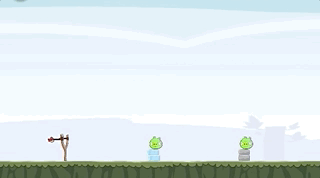
\includegraphics[width=0.23\textwidth]{images/double1.png}
% 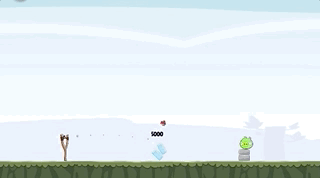
\includegraphics[width=0.23\textwidth]{images/double2.png}
% 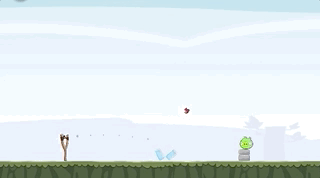
\includegraphics[width=0.23\textwidth]{images/double3.png}
% 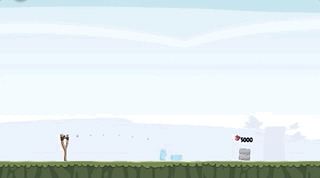
\includegraphics[width=0.23\textwidth]{images/double4.png}
% \end{center}
% \caption{Two pigs-one bird plan in execution.}
% \label{fig:double-hit}
% \end{figure*}

% \begin{figure*}
% \begin{center}
% 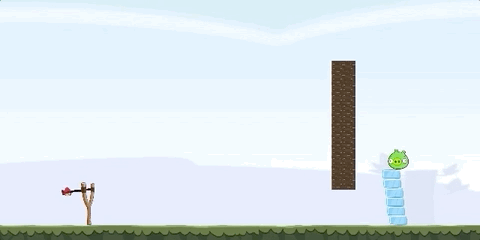
\includegraphics[width=0.23\textwidth]{images/under1.png}
% 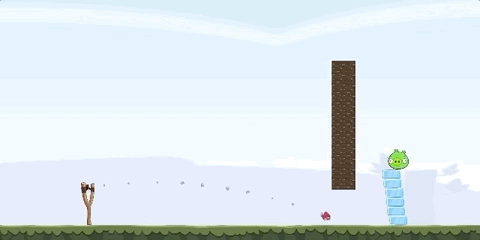
\includegraphics[width=0.23\textwidth]{images/under2.png}
% 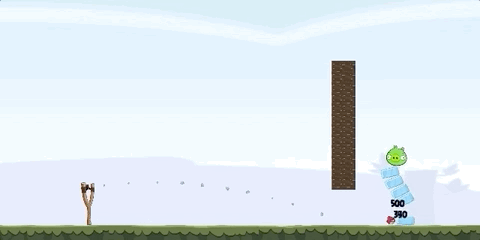
\includegraphics[width=0.23\textwidth]{images/under3.png}
% 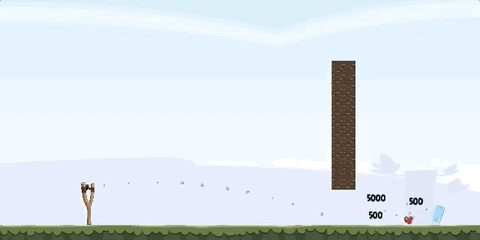
\includegraphics[width=0.23\textwidth]{images/under4.png}
% \end{center}
% \caption{Solution requiring bouncing of the ground and collapsing a structure to kill the target pig.}
% \label{fig:bounce-hit}
% \end{figure*}

% \setlength{\belowcaptionskip}{0pt}
% \begin{figure}[!ht]
% \begin{center}
% % \begingroup
%     \fontsize{8pt}{10pt}\selectfont
% \begin{verbatim}
% (:event collision_ground
%   :parameters (?b - bird)
%   :precondition (and
%     (= (active_bird) (bird_id ?b))
%     (<= (y_bird ?b) 0)  )
%   :effect (and
%     (assign (y_bird ?b) 1)
%     (assign (vy_bird ?b)
%     (* (* (vy_bird ?b) -1)(ground_damper)))
%     (assign (bounce_count ?b)
%     (+ (bounce_count ?b) 1))) )
% \end{verbatim}
% % \endgroup
% \caption{Event modeling a bird bouncing off the ground.}
% \label{fig:ground-event}
% \end{center}
% \end{figure}

% \smallskip
% Most interactions in a level occurs between birds and blocks in the scene. Blocks form structures which act as a protection barrier for targeted pigs. Thus, modeling collisions with blocks is vital to an accurate representation of Angry Birds. However, similarly to pig collisions, we opt to only define the event's effects in terms of the impact it has on the bird's velocity and the blocks stability and life values. There are two separate events modeling bird-block collisions with the distinction based on whether the block is stable enough to withstand the impact without being knocked out of place or destroyed entirely. In such cases, the bird bounces back off the block, otherwise it continues moving forward though with a diminished velocity.

% We decided that modeling the motion of blocks after impact, and chains of block-block collisions, using continuous dynamics would be prohibitively difficult. Such endeavor would require a significant implementation effort, defining a process for tracking each individual block's change in position and rotation over time, as well as a set of events to account for secondary interactions. These additions would only marginally improve the domain's accuracy, though the planner would experience a drastic drop in performance, having to keep track of dozens of simultaneous non-linear processes in every state after a collision.

% An additional event is present in the domain to account for a special case of block-block interactions, namely dislodging or destroying blocks supporting larger structures. In such cases, an event is triggered for every supported block, reducing its stability value to 0, repositioning the block to the ground, and adjusting its life value to account for fall damage. Analogously, we defined another event for killing pigs which sit atop of collapsing block structures. Figure~\ref{fig:bounce-hit} showcases the execution of a plan which includes a ground-bounce event, followed by the collapse of a tall structure to kill an otherwise unreachable target pig.

% The two final block-related events concern exploding TNT crates. Any impact upon the crate causes an explosion destroying all objects in its immediate vicinity and displacing objects further away. In our PDDL+ model, we incorporate two simple events modeling the explosive destruction of pigs and blocks nearby a TNT crate. As previously indicated, we omit the movement of objects caused by the explosion.

% The described events account for a significant portion of interactions during gameplay where birds are used to destroy multi-block structures to expose or kill targeted pigs, when a direct hit is infeasible or impossible.

% Platforms are indestructible objects which the agent needs to reason with to avoid poor results. However, almost no meaningful interactions occur between birds and platforms, and thus our domain contains an event modeling this type of collision but only to discourage the agent from shooting at platforms. The event deters the agent by nullifying the bird's velocity and expiring it without any impact on the level.

% Finally, we encode a supporting event which models the end of life for an active bird. In the game, a bird expires when it moves beyond the limits of the scene or when it stops moving. Modeling the exact timing of the end of a birds life is quite difficult. Instead, we define the birds usefulness in terms of the number of bounces off other objects. Each bounce partially reduces the bird's momentum, and its collision impact becomes negligible after three bounces. Therefore, we define a termination event for the active bird once it has bounced three times. The result of this event is that the next bird can be placed on the slingshot for launch.



% \setlength{\belowcaptionskip}{-10pt}
% \begin{table}[h]
% \centering
% \scriptsize
% \resizebox{\columnwidth}{!}{%
% \begin{tabular}{c|c|c|c|c|}
% \cline{2-5}
%  & \textbf{PDDL+} & \textbf{PDDL2.1} & \textbf{PDDL2.2} & \textbf{FSTRIPS+} \\ \hline
% \multicolumn{1}{|c|}{Bird Flight}              & $\checkmark$ & $\circ$ &  & $\checkmark$ \\ \hline
% \multicolumn{1}{|c|}{Collisions}               & $\checkmark$ &   & $\checkmark$   & \\ \hline
% \multicolumn{1}{|c|}{Explosions}               & $\checkmark$ &   & $\checkmark$   & \\ \hline
% \multicolumn{1}{|c|}{Structure collapse}       & $\checkmark$ &   & $\checkmark$   & \\ \hline
% \end{tabular}%
% }
% \caption{Language support for crucial Angry Birds features.}
% \label{tab:lang-comparison}
% \end{table}

% \smallskip
% To further solidify out choice of PDDL+ for modeling Angry Birds, table~\ref{tab:lang-comparison} shows an overview of relevant languages' ability to model crucial features of Angry Birds (note that PDDL2.1 can model the non-linear dynamics of flight but only as a durative action). As can be seen, only PDDL+ has the capacity to model and reason with all elements and dynamics of the game. Understanding the challenges of planning with such feature-rich models enabled us to make informed design decisions and preemptively mitigate any risks associated with PDDL+.



% \subsubsection*{Science Birds and the Hydra Agent}

% Our PDDL+-based game-playing agent, called Hydra, is designed to work with the Science Birds API~\cite{renz2015aibirds}. This API provides the game levels to the agents as a list of labeled objects and their locations.
% Hydra automatically translates this list into a PDDL+ problem file, which encodes the relevant information about this level. To solve these PDDL+ problems, we used UPMurphi~\cite{della2009upmurphi}, which is domain-independent PDDL+ planner that solves hybrid planning problems via a uniform discretization approach.

% While the goal of Angry Birds is to destroy all of the pigs, finding a solution to the corresponding PDDL+ problem was too difficult for our PDDL+ solver in some cases.
% Therefore, we considered two simplified problems:
% (1) a \textit{simplified problem}, which splits the original scenario into single-bird episodes with the goal of killing at least one pig, and (2) a \textit{relaxed simplified problem}, which only considers platforms and pigs.  plans for the simplified planning problem. If no plan is found in 30s,  relaxed simplified problem.
% If again, no plan is found in 30s, we execute a default non-planning action.


% was the best available planner and chose it for our evaluation.


% The choice of PDDL+ planner for our agent was motivated by the capabilities and performance of available software. The Angry Birds domain requires a high-performing planner able to handle large numbers of happenings, wide range of model features, and non-linear system dynamics.

% SMTPlan+~\cite{cashmore2016compilation} is a recent planner able to reason with all features of PDDL+ but it is only capable of dealing with polynomial non-linearity and does not scale well with the number of happenings. UPMurphi~\cite{della2009upmurphi} is a highly optimized PDDL+ planner which solves hybrid planning problems via a uniform discretization approach. UPMurphi can reason with the entire set of PDDL+ features and non-linear dynamics, though it is limited in performance by lack of heuristics. DiNo~\cite{piotrowski2016heuristic} is a PDDL+ planner which builds on the strengths of UPMurphi and extends it by implementing a domain-independent heuristic. However, DiNo's heuristic is computationally expensive and does not perform well on the Angry Birds domain, defeating its purpose. ENHSP~\cite{scala2016interval} is a planner for numeric domains equipped with an efficient heuristic. However, it can only handle problems encoded using the hybrid systems extension of FSTRIPS language which, as described before, is insufficiently expressive to model the Angry Birds domain. With that in mind, we concluded that UPMurphi was the best available planner and chose it for our evaluation.


%removedVspace

\begin{table}[tb!]
\centering
% \small
\begin{tabular}{|c|c|c|}
\hline
\textbf{Agent} & \textbf{Problems Solved} & \textbf{Avg. Score per Level} \\ \hline
ANU    & \textbf{49}              & 45,112                      \\ \hline
Hydra          & 44                       & \textbf{47,516}             \\ \hline
DataLab        & 26                       & 46,668                      \\ \hline
Eagle's  Wing  & 16                       & 39,152                      \\ \hline
\end{tabular}
\caption{Levels solved and avg. scores given a 60 sec. time limit.}
%removedVspace
\label{tab:results}
\end{table}

%The yearly Angry Birds competition~\cite{renz2015aibirds} at IJCAI ran by researchers from ANU yielded a number of game-playing AI agents. In this section,

% We evaluated Hydra against 3 agents:
% DataLab~\cite{borovicka2014datalab},
% Eagle's Wing~\cite{wang2017description}, and a baseline agent created by ANU.
% DataLab is the 2014 \& 2015 champion, whose actions are based on predicted utility of pre-defined strategies (destroy pigs, target TNT, target round blocks, destroy structures). Eagle's Wing is the 2016-2018 champion, which selects from 5 predefined strategies (pigshooter, TNT, most blocks, high round objects, and bottom building blocks), based on predicted utility. Eagle's Wing supplements these strategies with a trained XGBoost model to optimize its performance.
% The ANU agent targets a randomly selected pig with each active bird, and has predefined windows for tap actions per bird type. This agent only considers the locations of visible pigs, disregarding all other objects in the scene.


DataLab~\cite{borovicka2014datalab}, and
Eagle's Wing~\cite{wang2017description}.
DataLab won the 2014 \& 2015 ScienceBirds competition and Eagle's Wing won the 2016-2018 competitions.
Both agents work by trying a set of pre-defined strategies (e.g., destroy pigs, target TNT, target round blocks, destroy structures) and choosing the strategy that will yield the maximal predicted utility.
Eagle's Wing also uses a pre-trained XGBoost model to optimize its performance. %The ANU agent targets a randomly selected pig with each active bird, and has predefined windows for tap actions per bird type. This agent only considers the locations of visible pigs, disregarding all other objects in the scene.
All agents are designed to work with the ScienceBirds API. For the evaluation, each agent attempted to solve a set of 100 randomly generated Angry Birds levels, which can be found at~\emph{gitlab.com/aibirds/sciencebirdsframework} (for a fair comparison, all agents ran on the same set of levels).
We compared the results of all agents to a baseline performance published by ANU, which was computed by averaging the scores of
DataLab,
Eagle's Wing,
and an ANU-created naive agent.
The latter targets a randomly selected pig with each active bird, and has predefined windows for apply special actions per bird type. It only considers the locations of pigs, disregarding all other objects in the scene.


% developed using ANU's level generator\footnote{We used existing levels generated by ANU, which can be found at~\url{https://gitlab.com/aibirds/sciencebirdsframework/}}.
% As can be seen from the overall results (Tab.\ref{tab:results}), the Naive agent performed best overall solving 49 problems, followed closely by our HYDRA approach on 44 problems solved. Surprisingly, both Datalab and Eagle's Wing agents significantly underperformed on the evaluation test set, solving 26 and 16 problems, respectively.


Table~\ref{tab:results} shows the number of problem solved (out of 100) and the average score per level for each agent and the published baseline results (labelled ``ANU'').
As can be seen, Hydra's performance is on par with existing domain-dependent approaches, even without encoding the birds' special powers. It solved more problems than DataLab and Eagle's Wing (44 vs. 26 and 16) and obtained the highest average score (47,516) per level.
It is worth noting that both Eagle's Wing and DataLab's were designed for the ScienceBirds competition, where the levels were hand-crafted with specific winning strategies. In contrast, the levels we used were created by ANU's automated level generator.



% Fig.~\ref{fig:scores-plot} plots each agent's scores for each level in the evaluation. Levels are sorted on the $x$ axis by Hydra's scores.
% The line labelled ``ANU'' depicts baseline performance published by ANU,
% computed by averaging the scores of
% DataLab,
% Eagle's Wing,
% and an ANU-created naive agent.
% The latter targets a randomly selected pig with each active bird, and has predefined windows for tap actions per bird type. It only considers the locations of visible pigs, disregarding all other objects in the scene.
% As can be seen, Hydra's performance is on par with existing domain-dependent approaches, even without encoding the birds' special powers.
% Moreover, Hydra obtained the highest average score (47,516) per level.
% It is worth noting that both Eagle's Wing and DataLab's were designed for the ScienceBirds competition, where the levels were hand-crafted with specific winning strategies. In contrast, we evaluated them on levels created by an automated generator.
% %, lacking depth to effectively reason with level composition.



%The API provides the game levels to the agents as a list of labeled objects and their locations.
% Our agent supplements the ground truth information with our own deduced knowledge of the game and its objects. These are then merged and automatically translated into a PDDL+ problem file, encoding the collective relevant information about each level.


% \setlength{\belowcaptionskip}{-12pt}

% \begin{table}[ht!]
% \centering
% % \small
% \begin{tabular}{|c|c|c|}
% \hline
% \textbf{Agent} & \textbf{Problems Solved} & \textbf{Avg. Score per Level} \\ \hline
% Naive (ANU)    & \textbf{49}              & 45,112.4                      \\ \hline
% HYDRA          & 44                       & \textbf{47,515.7}             \\ \hline
% DataLab        & 26                       & 46667.8                      \\ \hline
% Eagle's  Wing  & 16                       & 39152.0                      \\ \hline
% \end{tabular}
% \caption{Evaluation results (solved levels and avg. scores).}
% \label{tab:results}
% \end{table}

% \subsection{Evaluation Results}


% \setlength{\belowcaptionskip}{-5pt}

% \begin{figure}[htbp!]
% % \begin{center}
% % 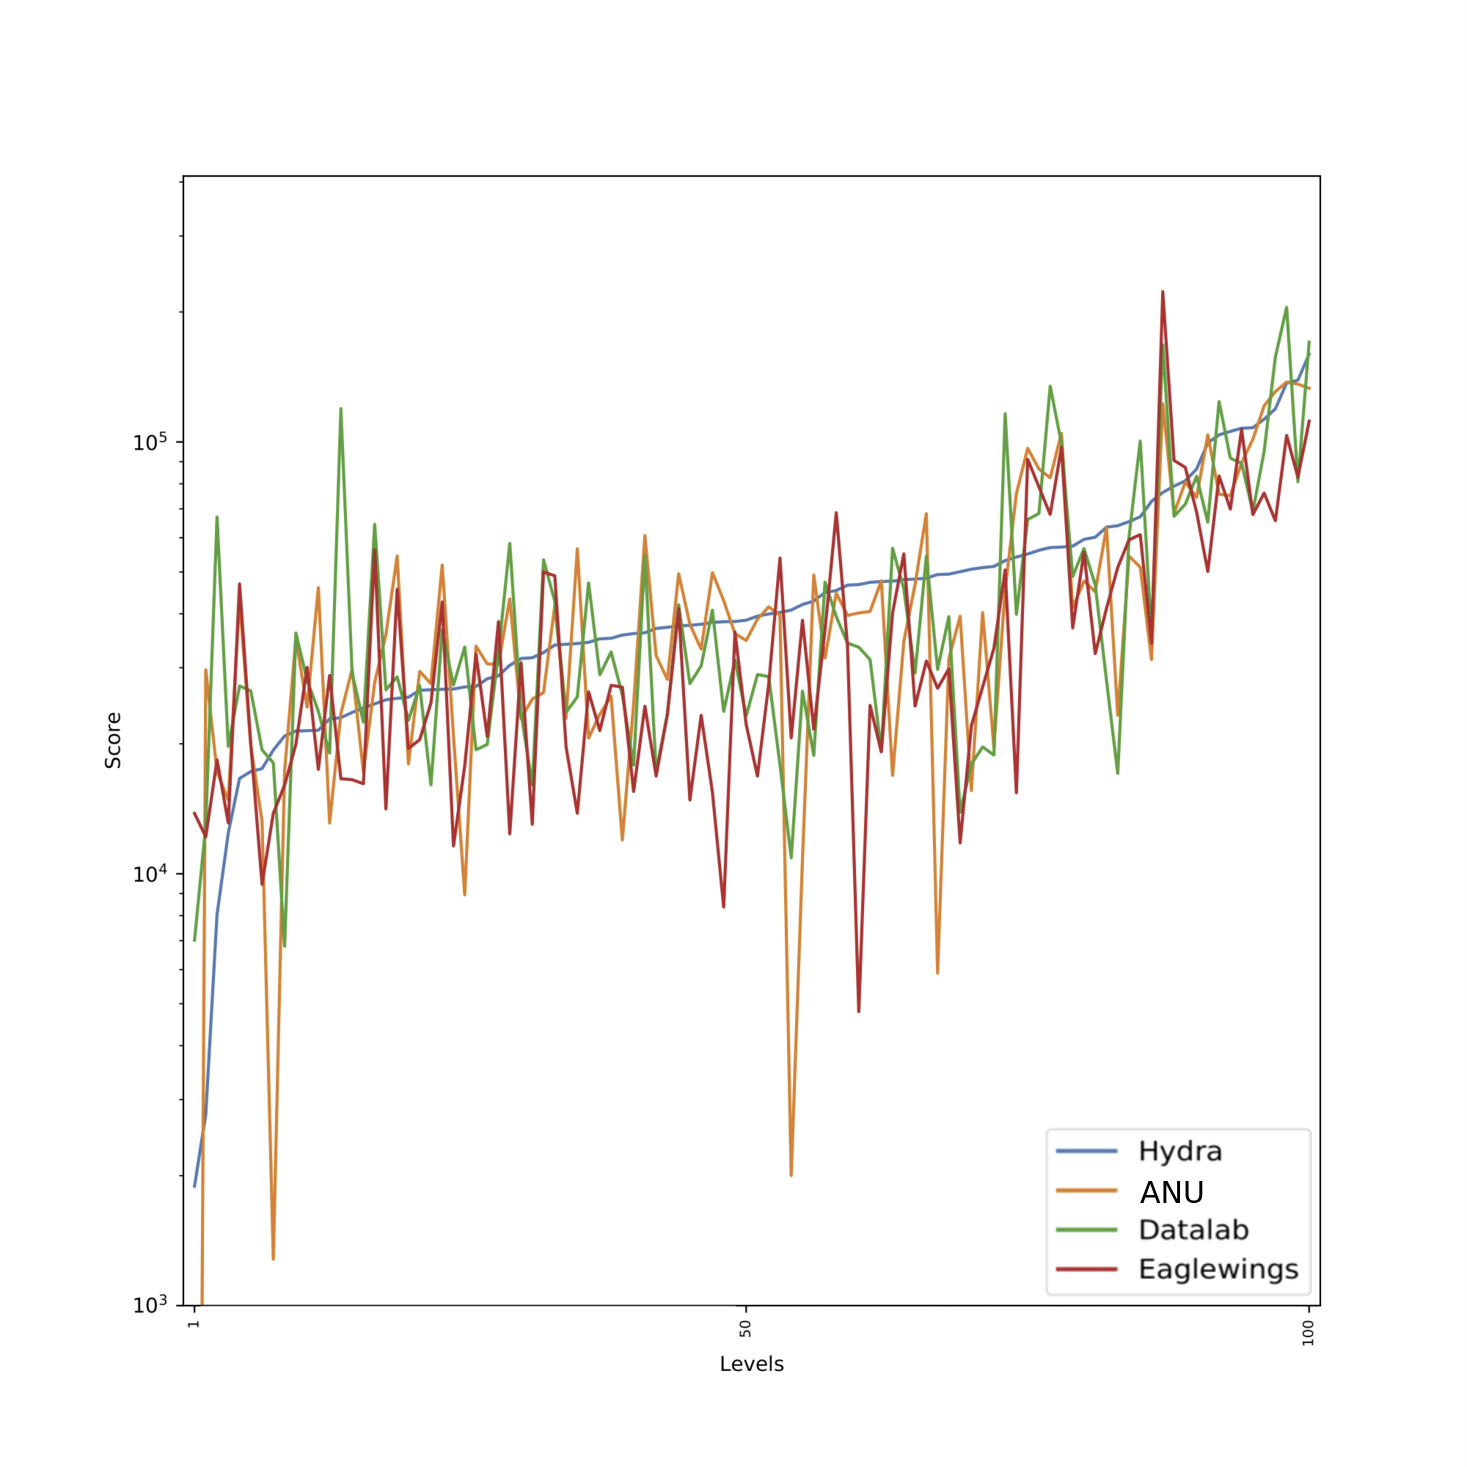
\includegraphics[trim= 50 45 50 82, clip, width=0.44\textwidth]{hydra-results-sb.png}
% % \end{center}
% \centering
% 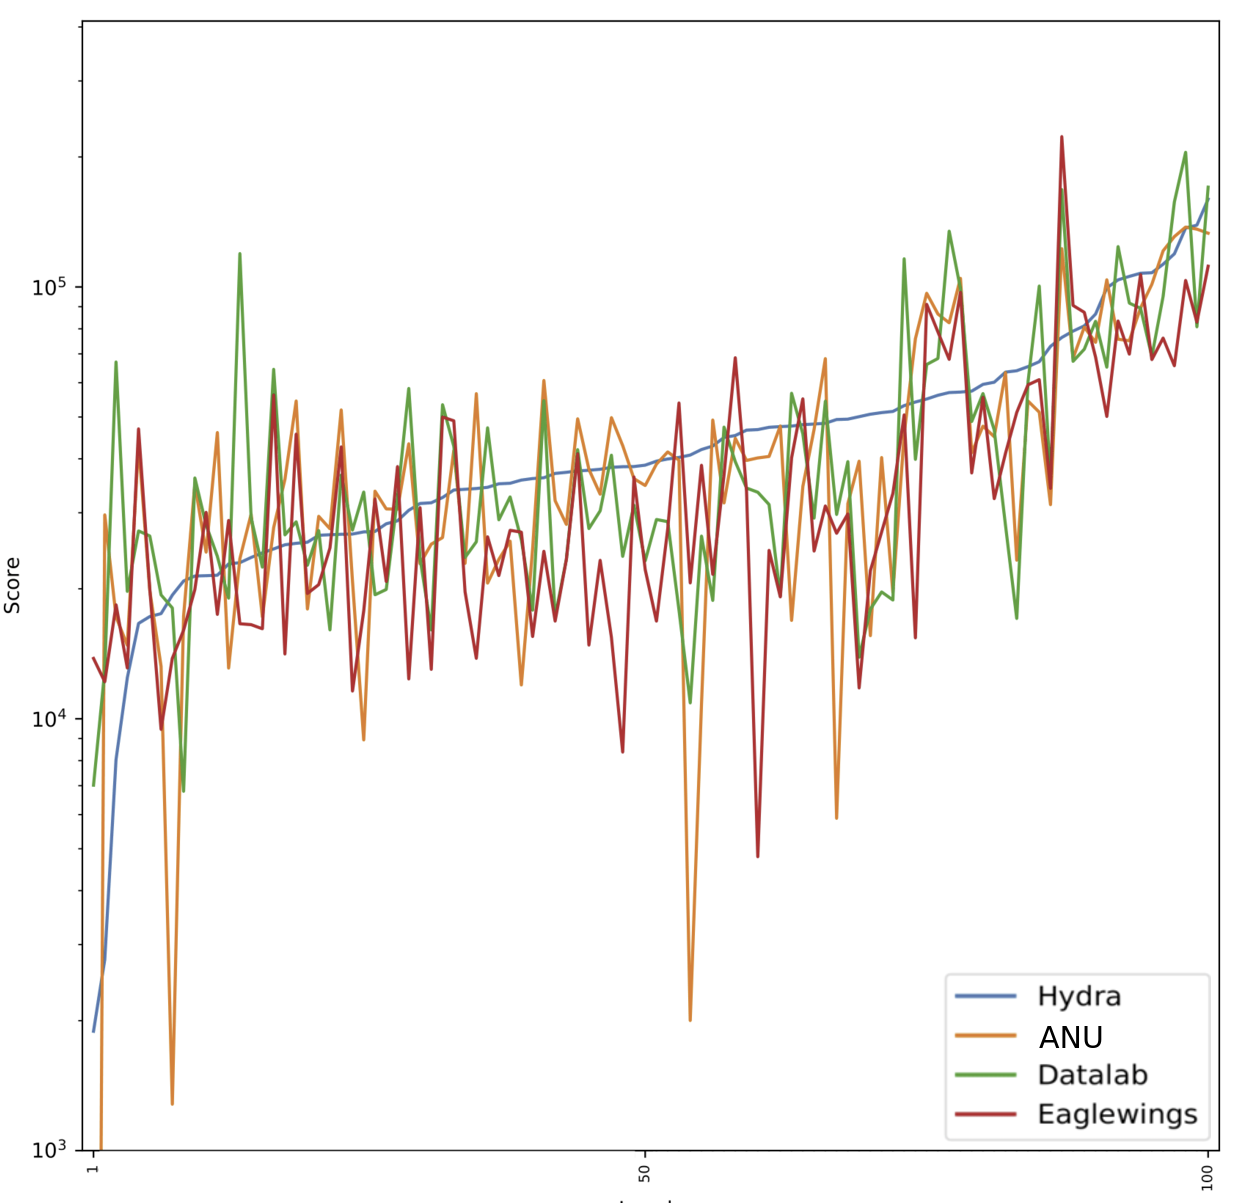
\includegraphics[width=0.65\columnwidth]{hydra-results-sb-cropped.png}
% \caption{Points per level, sorted by Hydra's scores.}
% \label{fig:scores-plot}
% \end{figure}

%Surprisingly, Datalab achieved an average score of 46667.8, outscoring the Naive agent (45112.4 points), even though the former solves significantly fewer levels. \Roni{Not so suprising, since it is the average score}
% The speculative cause for Eagle's Wing and DataLab's low performance might be attributed to the fact that the AI competition tested on hand-designed Angry Birds levels with specific winning strategies devised by their creators. Both agents rely on human devised strategies which proved to work well on the original Angry Birds levels but struggle to solve levels created by an automated generator. %, lacking depth to effectively reason with level composition.

% To determine if computational resources played a significant role in our performance, we report the number of shots performed as a result of different planning problems. Out of 358 possible shots in the evaluation only 34 used the relaxed simplification, and 30 employed the default non-planning action strategy. This indicates that one could improve performance through either a more accurate PDDL+ encoding of Angry Birds, or PDDL+ planner heuristics to tackle the full goal planning problems. We intend to pursue both courses of action in future phases of our research.

% One observation from the evaluation is that ANU's level generator produces compositions that rarely require advanced reasoning about the level's structure. Many of the generated levels can be  solved by only targeting pigs, as proved by the results of our experiments where the Naive agent outperformed sophisticated strategies of Eagle's Wing and Datalab. In future experiments we will aim to compose a set of test levels which require more diverse reasoning and strategies to achieve high scores.

\section{Conclusion}


% The success of Hydra in playing Angry Birds demonstrates

% We presented Hydra, which is an agent that plays the Angry Birds.

% We presented an agent that uses a domain-independent planner to successfully play Angry Birds, one of the most popular mobile games and a challenging AI testbed.
% It requires a highly expressive modeling language to capture  dynamics of the system. We determined the best way to accurately modeling the game as a planning domain is with PDDL+, an advanced planning language developed for hybrid systems.
% PDDL+ introduced a standardized method for including exogenous activity in planning domains via discrete events and continuous processes, which are critical to modeling Angry Birds' fundamental features.
% Next, we showed how leveraging the expressiveness of PDDL+ can mitigate its inherent risks and complexity while maintaining planning efficiency. Our evaluation showed promising results, with our agent (HYDRA) reaching the overall highest average score per level and significantly outperforming multiple champions of the Angry Birds AI competition.
%We presented an agent that successfully plays the popular and challenging Angry Birds game by using a domain-independent planner.
We presented an agent that successfully plays the Angry Birds game  using a domain-independent planner.
%To model this complex domain, our agent translates Angry Birds levels to PDDL+ problems and solves them using a PDDL+ solver.
Our agent translates Angry Birds levels to PDDL+ problems and solves them using a PDDL+ solver.
This demonstrates the expressive power of PDDL+ and corresponding solvers.
We plan on further extending our domain to improve its accuracy cient PDDL+ planning.
In addition, we are exploring techniques to diagnose incorrect PDDL+ models and repair them automatically~\cite{klenk2020model}.

% and repair complex
% [RONI: WANT TO PLUG THIS BUT NOT SURE WHERE] The Angry Birds domain differs from more typical PDDL+ applications in that the vast majority of system dynamics is defined via exogenous activity, and thus existing PDDL+ heuristics are less effective.


% , showing it can be used to model and solve challenging AI problem.
% We argue that PDDL+ is currently severely underused due to modeling complexity and large search spaces. However, we have shown that the expressiveness of PDDL+, in fact, facilitates building of efficient models which can mitigate these issues and enable solving of interesting and important problems.


%%%%%%%%

% \small
Adipisci aut nobis minus deserunt unde quia provident quis atque, aperiam a suscipit numquam aspernatur, tempore sunt aperiam numquam?Quo blanditiis perferendis, adipisci quod debitis deserunt soluta quo quos, fugit ipsa ipsum inventore.Suscipit quasi consequatur cum eius ea est cumque aliquam blanditiis, voluptatem ratione ex quia.Facilis quod nobis neque exercitationem, consequuntur facere quos voluptatum obcaecati sequi, accusantium delectus rem architecto quae nisi eveniet deserunt rerum perferendis culpa, nulla dolore vitae quia tempora magnam, cupiditate qui earum sed fugiat tempora adipisci ratione provident.Modi aliquam aut eveniet ea nam at fugiat, aut exercitationem veritatis fugit voluptate repudiandae beatae doloribus dolorum, repudiandae adipisci neque illum ea nihil tempore aliquid nisi quam laudantium, autem reprehenderit fugit?Vel sunt facere sint illo eligendi porro, in quasi velit reprehenderit, totam quos tenetur nulla impedit?Nam dolorem similique nesciunt reiciendis tempore vel maxime debitis voluptate harum facilis, quaerat sunt velit ipsam rem consequatur consectetur dolorum in, amet at sunt nulla voluptatem vitae architecto dicta earum?Eveniet sed non quos, consectetur velit vero similique quos cumque.Fugiat optio repellat, saepe et repellat nulla a tempore officiis nam labore praesentium minus, et rerum quia dignissimos minus ipsa doloribus recusandae id sed adipisci amet, asperiores atque reprehenderit exercitationem animi temporibus totam assumenda neque adipisci itaque.Temporibus cumque aliquid ad maiores saepe optio, sint tempora iste, delectus consectetur veritatis perferendis repellendus facere accusantium reprehenderit nobis amet at, architecto veniam eum?\clearpage
\bibliography{main}
\end{document}